\section{global.h File Reference}
\label{global_8h}\index{global.h@{global.h}}


This graph shows which files directly or indirectly include this file:\begin{figure}[H]
\begin{center}
\leavevmode
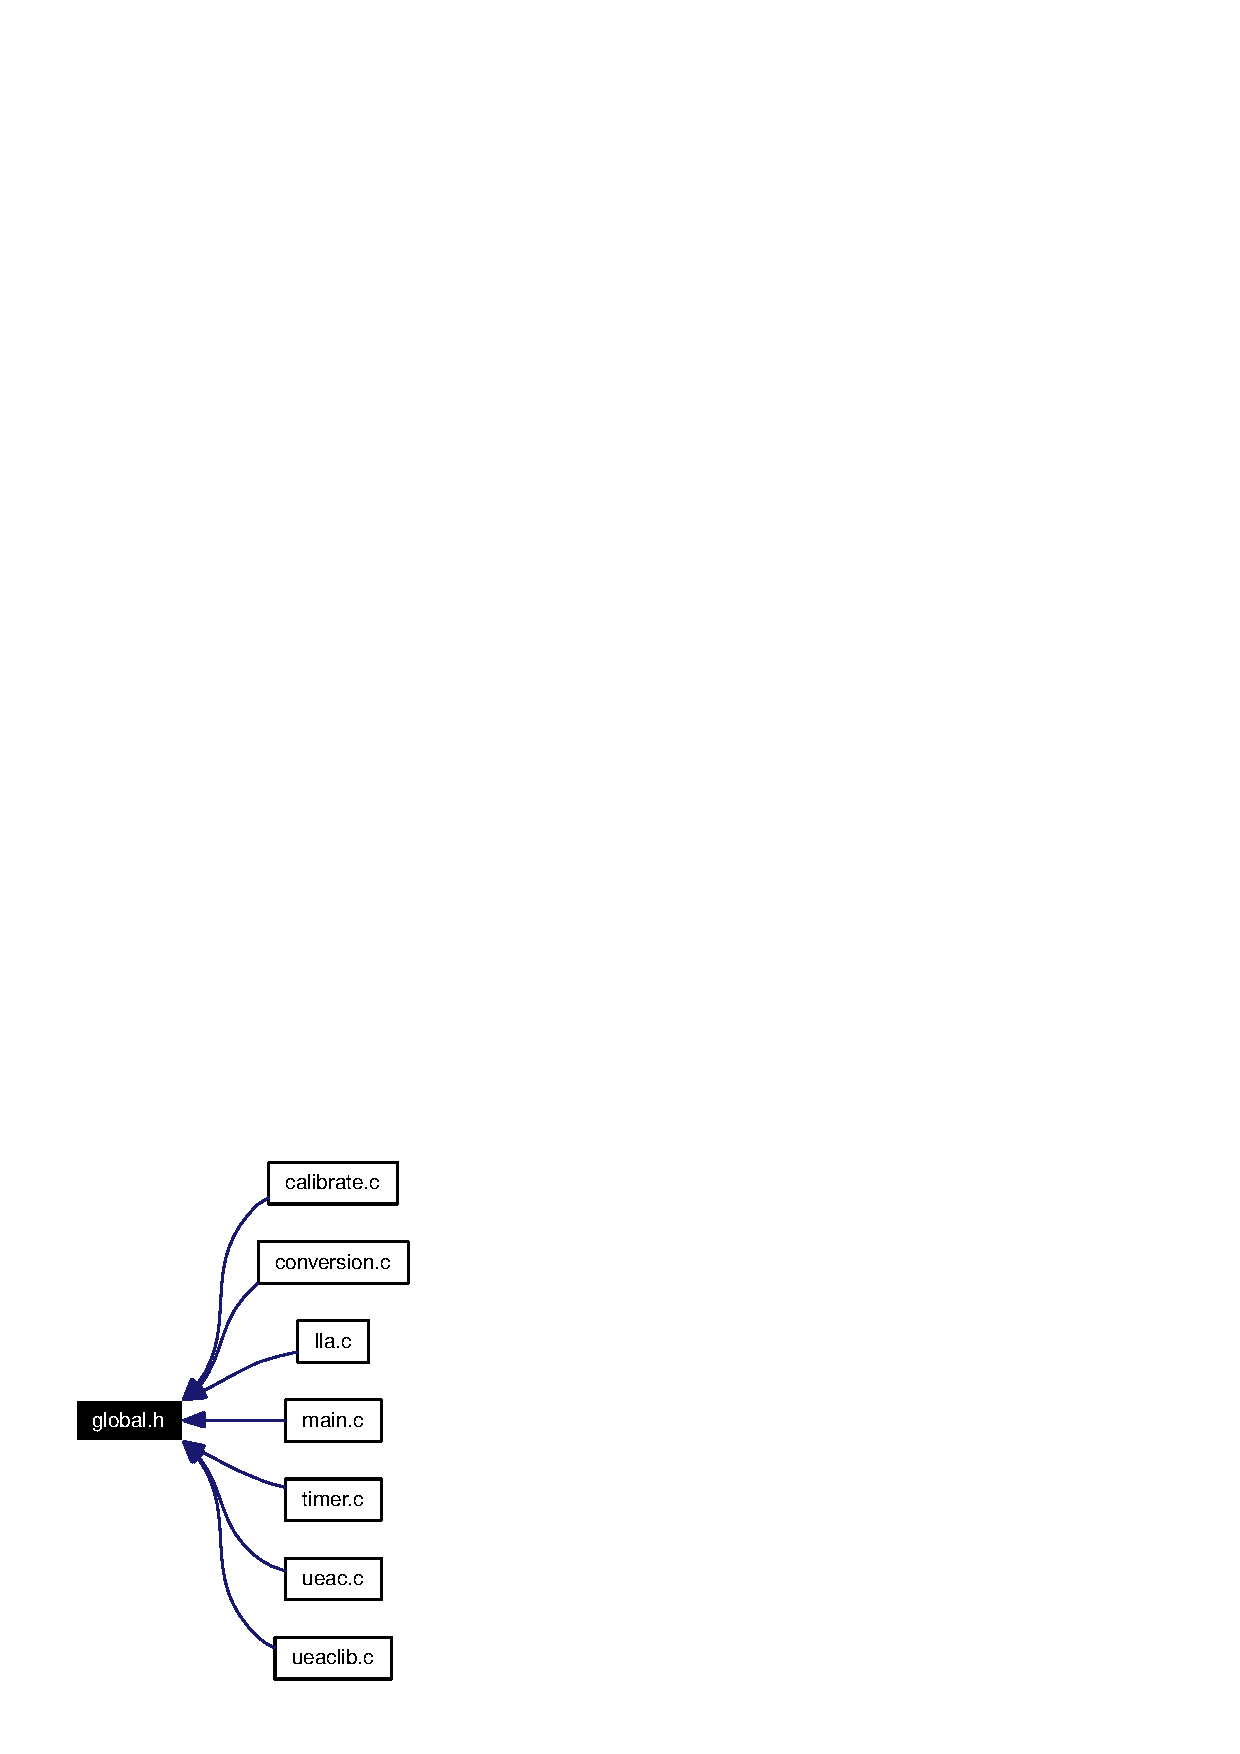
\includegraphics[width=98pt]{global_8h__dep__incl}
\end{center}
\end{figure}
\subsection*{Functions}
\begin{CompactItemize}
\item 
void {\bf init\_\-global\_\-variables} (void)
\end{CompactItemize}
\subsection*{Variables}
\begin{CompactItemize}
\item 
{\bf ueac\_\-t} {\bf ueac\_\-state}
\item 
char {\bf command} [100]
\item 
{\bf channel\_\-t} {\bf pin\_\-data} [25]
\item 
{\bf ueacval\_\-t} {\bf conversion\_\-result}
\item 
volatile int {\bf timer\_\-tick}
\item 
unsigned char {\bf led\_\-screen\_\-enable}
\item 
unsigned char {\bf high\_\-time\_\-limit} [25]
\end{CompactItemize}


\subsection{Function Documentation}
\index{global.h@{global.h}!init_global_variables@{init\_\-global\_\-variables}}
\index{init_global_variables@{init\_\-global\_\-variables}!global.h@{global.h}}
\subsubsection{\setlength{\rightskip}{0pt plus 5cm}void init\_\-global\_\-variables (void)}\label{global_8h_a7}




Definition at line 121 of file global.c.

References init\_\-pin\_\-data\_\-structure(), init\_\-ueac\_\-state\_\-structure(), led\_\-screen\_\-enable, and timer\_\-tick.

Referenced by main().

\footnotesize\begin{verbatim}121                                   {
122   init_pin_data_structure();   
123   init_ueac_state_structure();
124   timer_tick=0;
125   led_screen_enable=0;
126 }
\end{verbatim}\normalsize 




Here is the call graph for this function:\begin{figure}[H]
\begin{center}
\leavevmode
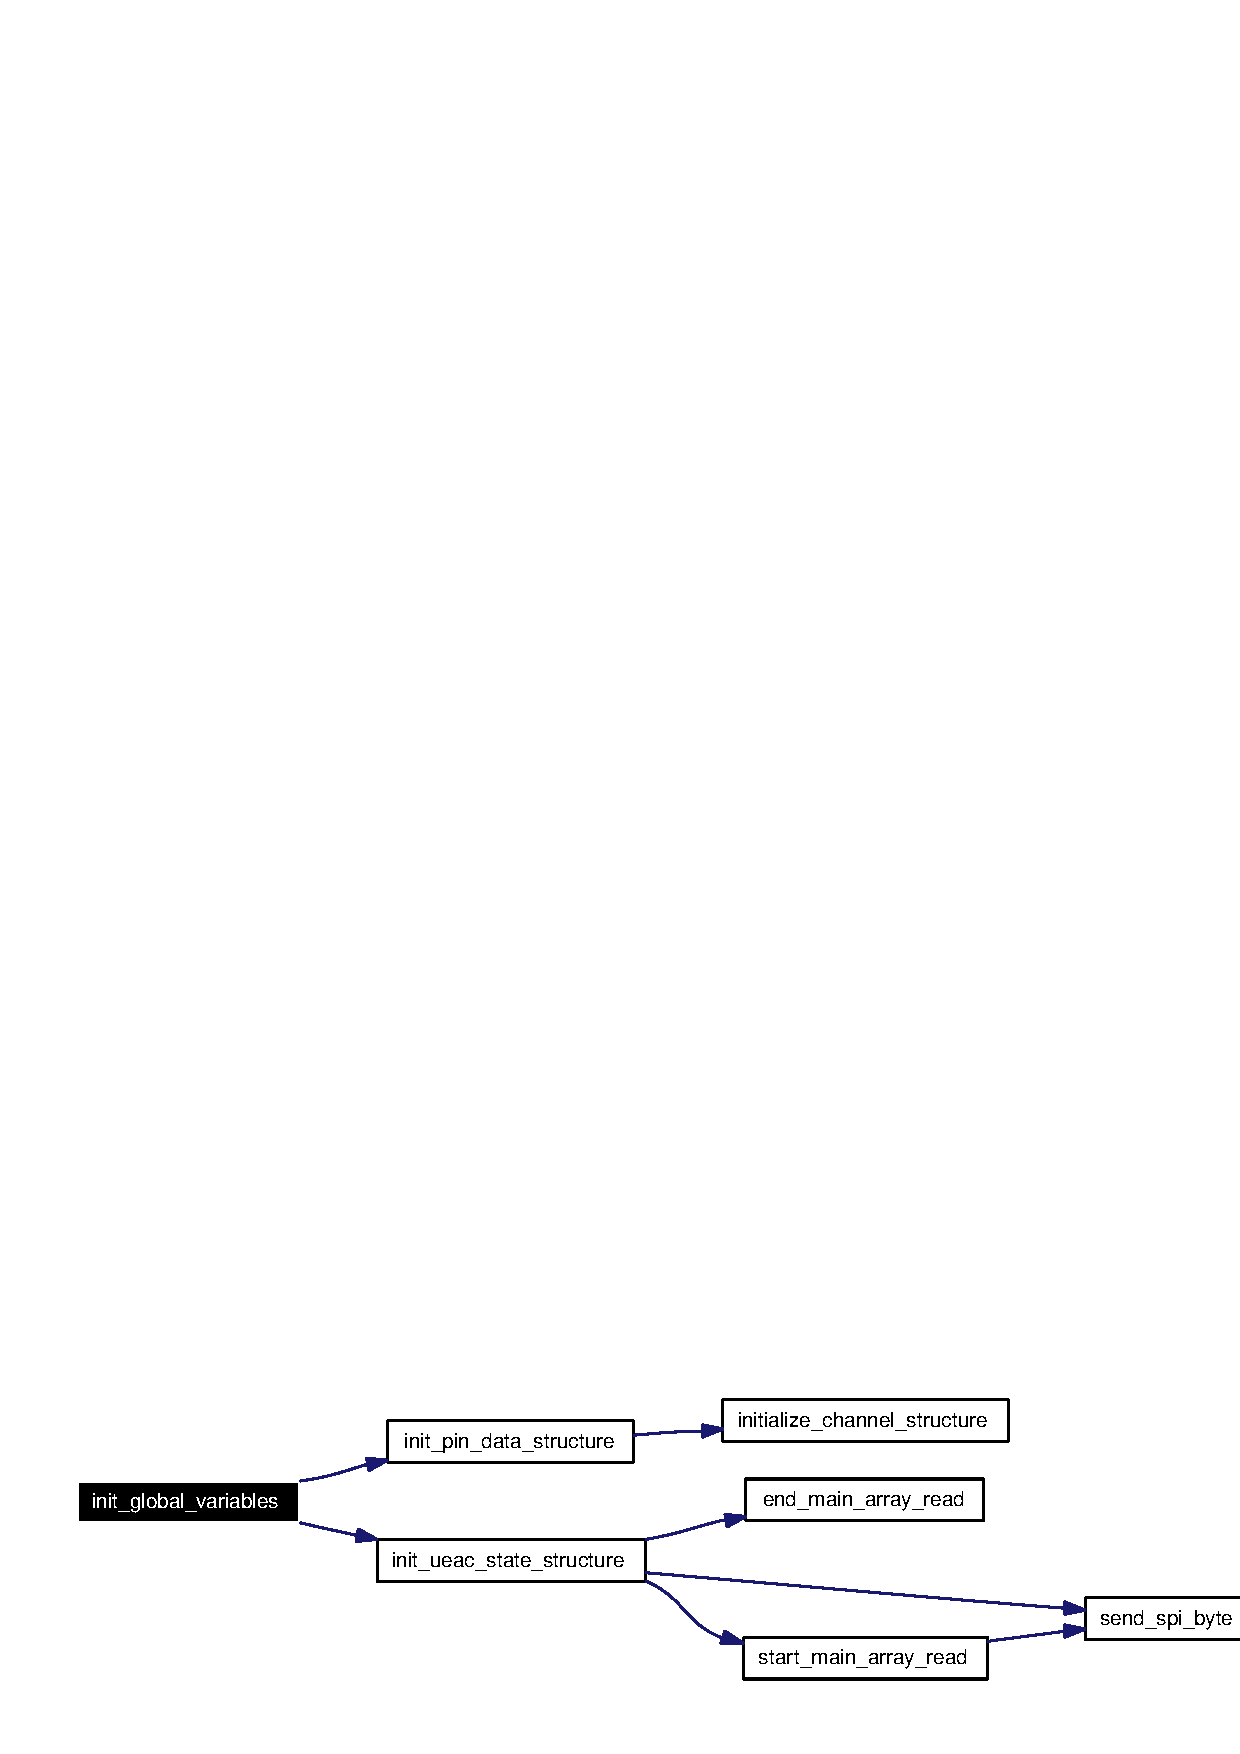
\includegraphics[width=301pt]{global_8h_a7_cgraph}
\end{center}
\end{figure}


\subsection{Variable Documentation}
\index{global.h@{global.h}!command@{command}}
\index{command@{command}!global.h@{global.h}}
\subsubsection{\setlength{\rightskip}{0pt plus 5cm}char {\bf command}[100]}\label{global_8h_a1}




Definition at line 55 of file global.c.

Referenced by main().\index{global.h@{global.h}!conversion_result@{conversion\_\-result}}
\index{conversion_result@{conversion\_\-result}!global.h@{global.h}}
\subsubsection{\setlength{\rightskip}{0pt plus 5cm}{\bf ueacval\_\-t} {\bf conversion\_\-result}}\label{global_8h_a3}




Definition at line 57 of file global.c.

Referenced by print\_\-grid\_\-i(), print\_\-grid\_\-v(), scan\_\-probes(), and ueac\_\-execute\_\-instruction().\index{global.h@{global.h}!high_time_limit@{high\_\-time\_\-limit}}
\index{high_time_limit@{high\_\-time\_\-limit}!global.h@{global.h}}
\subsubsection{\setlength{\rightskip}{0pt plus 5cm}unsigned char {\bf high\_\-time\_\-limit}[25]}\label{global_8h_a6}




Definition at line 60 of file global.c.

Referenced by led\_\-pwm(), and timer\_\-a0\_\-irq().\index{global.h@{global.h}!led_screen_enable@{led\_\-screen\_\-enable}}
\index{led_screen_enable@{led\_\-screen\_\-enable}!global.h@{global.h}}
\subsubsection{\setlength{\rightskip}{0pt plus 5cm}unsigned char {\bf led\_\-screen\_\-enable}}\label{global_8h_a5}




Definition at line 59 of file global.c.

Referenced by init\_\-global\_\-variables(), main(), timer\_\-a0\_\-irq(), and ueac\_\-execute\_\-instruction().\index{global.h@{global.h}!pin_data@{pin\_\-data}}
\index{pin_data@{pin\_\-data}!global.h@{global.h}}
\subsubsection{\setlength{\rightskip}{0pt plus 5cm}{\bf channel\_\-t} {\bf pin\_\-data}[25]}\label{global_8h_a2}




Definition at line 56 of file global.c.

Referenced by current\_\-output\_\-calibration(), evaluate\_\-lla(), print\_\-grid\_\-i(), print\_\-grid\_\-v(), scan\_\-probes(), timer\_\-a0\_\-irq(), and ueac\_\-execute\_\-instruction().\index{global.h@{global.h}!timer_tick@{timer\_\-tick}}
\index{timer_tick@{timer\_\-tick}!global.h@{global.h}}
\subsubsection{\setlength{\rightskip}{0pt plus 5cm}volatile int {\bf timer\_\-tick}}\label{global_8h_a4}




Definition at line 58 of file global.c.

Referenced by delay\_\-1\_\-25m\-S(), init\_\-global\_\-variables(), and timer\_\-a0\_\-irq().\index{global.h@{global.h}!ueac_state@{ueac\_\-state}}
\index{ueac_state@{ueac\_\-state}!global.h@{global.h}}
\subsubsection{\setlength{\rightskip}{0pt plus 5cm}{\bf ueac\_\-t} {\bf ueac\_\-state}}\label{global_8h_a0}




Definition at line 54 of file global.c.

Referenced by convert\_\-a2d(), main(), timer\_\-a0\_\-irq(), ueac\_\-execute\_\-instruction(), and write\_\-current().